% BraTS 2026 Challenge -- Task 1 (Brain Metastases) -- short paper
%
% RULES (verified 2026-07-28 against Synapse wiki syn74274097, page 639582):
%   * 8-10 pages WITHOUT references. Citations do not count toward the limit.
%   * Springer LNCS format (bit.ly/2TEcZNF).
%   * Mandatory sections, in order: Abstract (NO CITATIONS) / Keywords /
%     Introduction / Methods / Results / Discussion / Acknowledgements (optional) /
%     References (must include the citations listed in the Challenge Rules).
%   * Submit via OpenReview: https://openreview.net/group?id=MICCAI.org/2026/Challenge
%     (BraTS-METS subgroup: .../Challenge/BraTS-METS)
%   * You will be asked for the Synapse team name: 3495063
%
% Requires llncs.cls -- see paper/README.md.
\documentclass[runningheads]{llncs}

\usepackage{graphicx}
\usepackage{booktabs}
\usepackage{array}
\usepackage{amsmath}
\usepackage{tikz}
\usetikzlibrary{arrows.meta,positioning}
\usepackage{xcolor}
\usepackage[hidelinks]{hyperref}

\begin{document}

\title{Confident Mistakes: Hysteresis Decoding and the\\ Limits of False-Positive Suppression in\\ Brain Metastasis Segmentation}
\titlerunning{Confident Mistakes in Brain Metastasis Segmentation}

\author{%
Soumya Snigdha Kundu \and
Theodore Barfoot \and
Marina Ivory \and
Kabir Hamzah Muhammad \and
Lorena Garcia-Foncillas Macias \and
Jonathan Shapey \and
Tom Vercauteren%
}
\authorrunning{S. S. Kundu et al.}

\institute{School of Biomedical Engineering \& Imaging Sciences,\\
King's College London, London, UK\\
% TODO(verify): institutional e-mail address for the corresponding author.
\email{soumya\_snigdha.kundu@kcl.ac.uk}}

\maketitle

%%%%%%%%%%%%%%%%%%%%%%%%%%%%%%%%%%%%%%%%%%%%%%%%%%%%%%%%%%%%%%%%%%%%%%%%%%%%%%%
% ABSTRACT -- one paragraph, 6-7 sentences. NO CITATIONS (challenge rule).
\begin{abstract}
Brain metastasis segmentation is scored lesion-wise, which turns it into a detection problem:
each lesion counts equally regardless of volume, and every spurious component is charged twice,
once as a zero in the Dice average and once in the $F_1$ denominator. Most challenge effort goes
into architectures and losses. We find the decisive gains lie downstream, in how probabilities
become a label map, and we make three claims. First, an unweighted average of three nnU-Net
ResEnc-L variants decoded by hysteresis thresholding raises lesion-wise Dice from
0.560/0.622/0.593 to 0.725/0.766/0.746, with those two inference-time steps contributing over
four fifths of the gain and no new architecture, loss, or training run; hysteresis works because
it splits the decision of whether a lesion exists from how far it extends, and never inspects
component size. Second, the residual error is not separable by confidence: the median peak
probability inside our false positives is 0.96 against 0.55 inside the lesions we miss, and we
refute seven suppression mechanisms that all founder on this inversion. Third, post-processing
that changes how many components are retained cannot be validated on training cases at all, even
relatively, because a memorised model rarely emits the spurious components such a rule would
admit; this inverted the sign of one of our submissions, which measured $+0.028$ Dice offline and
delivered $-0.016$. For practitioners tuning lesion-wise systems, the second and third claims
bound what post-processing can achieve and mark a category of offline experiment whose results
should not be believed.

\keywords{Brain metastases \and Lesion-wise evaluation \and Ensembling \and Hysteresis
thresholding \and False positives \and nnU-Net \and BraTS.}
\end{abstract}

%%%%%%%%%%%%%%%%%%%%%%%%%%%%%%%%%%%%%%%%%%%%%%%%%%%%%%%%%%%%%%%%%%%%%%%%%%%%%%%
\section{Introduction}
\label{sec:intro}

Brain metastases are the most common intracranial malignancy, and their automated delineation
differs from glioma segmentation in a way that governs method design: the clinically decisive
targets are numerous, small, and scattered. The BraTS-MET task therefore scores
\emph{lesion-wise}~\cite{bratsmet2023}. Predicted components are matched one-to-one to reference
components~\cite{grosskopf2026matching}, each lesion contributes equally to the Dice and normalised surface Dice (NSD)
averages irrespective of volume, and an unmatched prediction is penalised twice---once as a zero
appended to the lesion-wise Dice average, and again in the denominator of small-instance $F_1$.

This inverts the usual economics. Under volumetric Dice a five-voxel false positive is
negligible; under lesion-wise scoring it costs as much as missing a large lesion. Conversely, a
method that suppresses small components to protect Dice destroys the detection metric the task
exists to measure. Over the operating range that matters the two objectives are not merely
distinct but opposed, and we quantify that opposition in Section~\ref{sec:frontier}.

We began from a standard nnU-Net ResEnc-L~\cite{isensee2021nnunet,isensee2024resenc} baseline and
found repeatedly that changes to the network bought less than changes to how its probabilities
became a label map. Our contributions are:

\begin{enumerate}
\item \textbf{An inference-time recipe that is most of our performance.} Ensembling as an
      explicit false-positive dilution mechanism, plus hysteresis decoding, contribute over
      four fifths of our total Dice improvement over the baseline
      (Section~\ref{sec:ablation}), with no new architecture, loss, or training run.
\item \textbf{A characterisation of the residual error, with seven refutations.} We show the
      remaining false positives are confident, coherent, isolated and corroborated across
      independently trained networks, and that seven suppression mechanisms---several of them
      standard practice---fail for this one reason (Section~\ref{sec:fp}).
\item \textbf{A negative result about offline threshold tuning.} We identify a class of
      post-processing rule that \emph{cannot} be validated on training cases even in a purely
      relative comparison, and demonstrate it inverting the sign of a real submission
      (Section~\ref{sec:harness}).
\end{enumerate}

\paragraph{What is and is not novel.} No component here is new: nnU-Net and its residual-encoder
variants are off the shelf~\cite{isensee2021nnunet,isensee2024resenc}, probability averaging is
standard, hysteresis dates to Canny~\cite{canny1986}, and our third member's objective follows
blob loss~\cite{kofler2022blob,kundu2026instance}. We claim the empirical finding that this combination is where
the performance is under lesion-wise scoring, plus the two negative results. Readers looking for
a new architecture will not find one, and our argument is that they should not be looking.

%%%%%%%%%%%%%%%%%%%%%%%%%%%%%%%%%%%%%%%%%%%%%%%%%%%%%%%%%%%%%%%%%%%%%%%%%%%%%%%
\section{Methods}
\label{sec:methods}

\subsection{Data}
\label{sec:data}

We use the BraTS-MET 2026 training set: 1295 multi-site cases, each with four co-registered,
skull-stripped sequences (T1, T1-Gd, T2, T2-FLAIR) supplied in \emph{native} space, so voxel
spacing and array dimensions vary across the cohort. Reference labels comprise non-enhancing
tumour core (NETC), surrounding non-enhancing FLAIR hyperintensity (SNFH), enhancing tumour (ET)
and resection cavity (RC). Region prevalence is markedly imbalanced---54\% NETC, 89\% SNFH,
96\% ET and only 13\% RC---which is the principal reason the RC channel is our weakest and is
handled separately below. Validation uses the official 179-case set scored on the challenge
server; we never see its reference labels.

We predict four \emph{overlapping} binary regions with independent sigmoids rather than mutually
exclusive classes,
\[
\mathrm{WT}=\{1,2,3\},\quad \mathrm{TC}=\{1,3\},\quad \mathrm{ET}=\{3\},\quad \mathrm{RC}=\{4\},
\]
decoded in the order WT $\rightarrow$ TC $\rightarrow$ ET $\rightarrow$ RC so nested regions
overwrite their parents. This is the \texttt{Dataset007} configuration in our released code.

\subsection{Ensemble members}
\label{sec:members}

The submission averages three ResEnc-L models sharing the residual-encoder plans and the
\texttt{3d\_fullres} configuration (Table~\ref{tab:members}), all trained on all available
data without a held-out fold---a decision we revisit critically in Sections~\ref{sec:harness}
and~\ref{sec:limits}.

\begin{table}[t]
\centering
\caption{Ensemble members. All are nnU-Net ResEnc-L, \texttt{3d\_fullres}, trained on all data.}
\label{tab:members}
\begin{tabular}{@{}llll@{}}
\toprule
member & data configuration & training objective & role in the ensemble \\
\midrule
TopK        & 4-region  & Dice + top-$K$ BCE          & high-precision base \\
completion  & 6-region  & Dice + top-$K$ BCE          & decorrelated second view \\
CC-loss     & 6-region  & component-weighted fine-tune & high-recall detector \\
\bottomrule
\end{tabular}
\end{table}

The third member is fine-tuned with a connected-component-aware objective that weights each
lesion equally rather than each voxel, following the blob-loss
principle~\cite{kofler2022blob,kundu2026instance}.
It is our strongest detector and our weakest segmenter. Submitted alone it reached small-instance
$F_1$ of .429/.530/.543, the highest we ever recorded, while its lesion-wise Dice fell to
.670/.715/.691, far below our baseline; alone, it is sunk entirely by its false positives. This
tension is precisely what the ensemble exploits.

Inference uses sliding-window prediction with \texttt{step\_size} 0.25 and test-time
augmentation by mirroring, retaining per-region probability maps.

\subsection{Ensembling as false-positive dilution}
\label{sec:ensembling}

The tumour probability map is the unweighted mean over members $m$,
\[
\bar{p}_r(x) \;=\; \tfrac{1}{3}\sum_{m=1}^{3} p_r^{(m)}(x), \qquad
r \in \{\mathrm{WT},\mathrm{TC},\mathrm{ET}\}.
\]

The mechanism is asymmetric, and the asymmetry is the point. A detection supported by all three
members retains a high mean; one idiosyncratic to a single member is divided by three and falls
below the decision threshold. Averaging the high-recall CC-loss member into two cleaner models
reduced false positives from \textbf{1.66 to 0.85 per case} while retaining its corroborated true
detections. Dice and $F_1$ rose \emph{together} rather than trading---the only mechanism we found
that does so, and the reason the ensemble is not merely a variance-reduction convenience.

The resection cavity is treated separately. RC is a single large structure for which ensembling
gave no benefit: a two-model RC average moved lesion-wise Dice from 0.630 to 0.628, within noise.
We therefore take RC from the CC-loss member alone, threshold at 0.5, and retain only the largest
connected component.

\subsection{Hysteresis decoding}
\label{sec:hysteresis}

Converting $\bar{p}$ to a mask with one global threshold $t$ forces a single number to answer two
unrelated questions. A low $t$ promotes every noise speck to a lesion; a high $t$ amputates every
real lesion at its margin, because the tumour boundary in these probability maps lies between
roughly 0.30 and 0.60. No single value is correct for both.

Hysteresis thresholding, borrowed from classical edge detection~\cite{canny1986}, splits the two
decisions across thresholds $lo < hi$. Writing $\mathcal{C}(\cdot)$ for the set of 26-connected
components of a binary mask, the decoded region is
\[
\hat{M} \;=\; \bigcup \Big\{\, c \in \mathcal{C}\big(\bar{p}_r > lo\big) \;:\;
\max_{x \in c} \bar{p}_r(x) > hi \,\Big\},
\]
that is, every component of the permissive mask whose \emph{peak} clears the strict threshold is
retained \emph{at its full permissive extent}. Figure~\ref{fig:hyst} illustrates the three cases
that matter.

\begin{figure}[t]
\centering
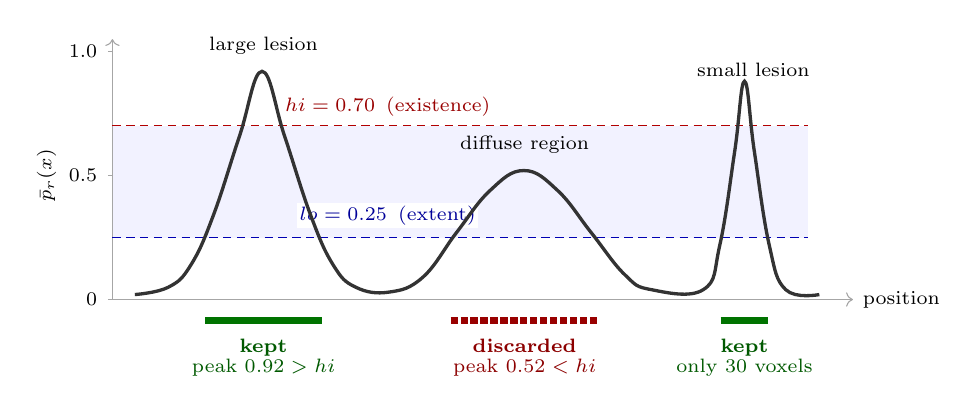
\begin{tikzpicture}[xscale=0.95, yscale=3.15]

% ---- threshold bands -------------------------------------------------------
\fill[blue!5]  (0,0.25) rectangle (9.3,0.70);

% ---- axes ------------------------------------------------------------------
\draw[->,gray!70] (0,0) -- (9.9,0) node[right,black,font=\scriptsize] {position};
\draw[->,gray!70] (0,0) -- (0,1.05);
\foreach \y/\l in {0/0, 0.5/0.5, 1.0/1.0}
  \draw[gray!70] (-0.06,\y) -- (0,\y) node[left,black,font=\scriptsize,xshift=-2pt] {\l};
\node[rotate=90,font=\scriptsize,anchor=south] at (-0.62,0.5) {$\bar{p}_r(x)$};

% ---- thresholds (labelled in the empty gap between the first two lesions) ---
\draw[densely dashed,red!70!black]  (0,0.70) -- (9.3,0.70);
\draw[densely dashed,blue!70!black] (0,0.25) -- (9.3,0.25);
\node[font=\scriptsize,red!60!black,anchor=south,fill=white,inner sep=1pt]
  at (3.68,0.725) {$hi=0.70$ \,(existence)};
\node[font=\scriptsize,blue!60!black,anchor=south,fill=white,inner sep=1pt]
  at (3.68,0.285) {$lo=0.25$ \,(extent)};

% ---- probability profile ---------------------------------------------------
\draw[very thick,black!80] plot[smooth,tension=0.7] coordinates {
  (0.30,0.02) (0.75,0.05) (1.05,0.14) (1.35,0.34) (1.70,0.66) (2.00,0.92)
  (2.30,0.66) (2.65,0.34) (2.95,0.14) (3.25,0.05) (3.70,0.03)
  (4.15,0.09) (4.60,0.27) (5.05,0.44) (5.50,0.52) (5.95,0.44) (6.40,0.27)
  (6.85,0.10) (7.20,0.04)
  (7.90,0.04) (8.12,0.22) (8.32,0.60) (8.45,0.88) (8.58,0.60) (8.78,0.22)
  (9.00,0.04) (9.45,0.02) };

% ---- retained / discarded extents ------------------------------------------
\draw[line width=2.6pt,green!45!black] (1.24,-0.085) -- (2.80,-0.085);
\draw[line width=2.6pt,red!60!black,densely dotted] (4.52,-0.085) -- (6.50,-0.085);
\draw[line width=2.6pt,green!45!black] (8.13,-0.085) -- (8.77,-0.085);

% ---- annotations -----------------------------------------------------------
\node[font=\scriptsize,align=center,green!35!black] at (2.02,-0.235)
  {\textbf{kept}\\[-1pt] peak $0.92>hi$};
\node[font=\scriptsize,align=center,red!55!black] at (5.51,-0.235)
  {\textbf{discarded}\\[-1pt] peak $0.52<hi$};
\node[font=\scriptsize,align=center,green!35!black] at (8.45,-0.235)
  {\textbf{kept}\\[-1pt] only 30 voxels};

\node[font=\scriptsize,anchor=south] at (2.02,0.95) {large lesion};
\node[font=\scriptsize,anchor=south] at (5.51,0.55) {diffuse region};
\node[font=\scriptsize,anchor=south east] at (9.45,0.86) {small lesion};

\end{tikzpicture}
\caption{Hysteresis decoding on a 1-D slice through the fused probability map; the shaded band
spans $lo$ to $hi$. Thresholding at $hi$ alone would keep only the peaks above the band,
amputating each lesion's margin; at $lo$ alone it would admit the diffuse region. Hysteresis keeps
every component of $\bar{p}_r>lo$ whose peak clears $hi$, at full $lo$-extent (green), and drops
those that never do (red). Size is never consulted, so the 30-voxel lesion survives on one
confident voxel while the far larger diffuse region does not.}
\label{fig:hyst}
\end{figure}

The critical property is what the rule does \emph{not} use. It thresholds on peak probability and
never on component size or mean probability. This is what separates it from the component filters
that fail here (Section~\ref{sec:fp}): size and mean confidence both correlate with \emph{being a
small true lesion}, so filtering on them preferentially destroys the targets the task rewards,
whereas peak probability does not. A thirty-voxel metastasis with a single voxel at 0.9 survives
intact; a large diffuse region never reaching 0.7 anywhere is removed in full. One confident
voxel is sufficient evidence of existence, and existence is what $F_1$ measures.

Hysteresis is applied per region to WT, TC and ET, and excluded for RC.

\subsection{Final pipeline and reproducibility}

\begin{figure}[t]
\centering
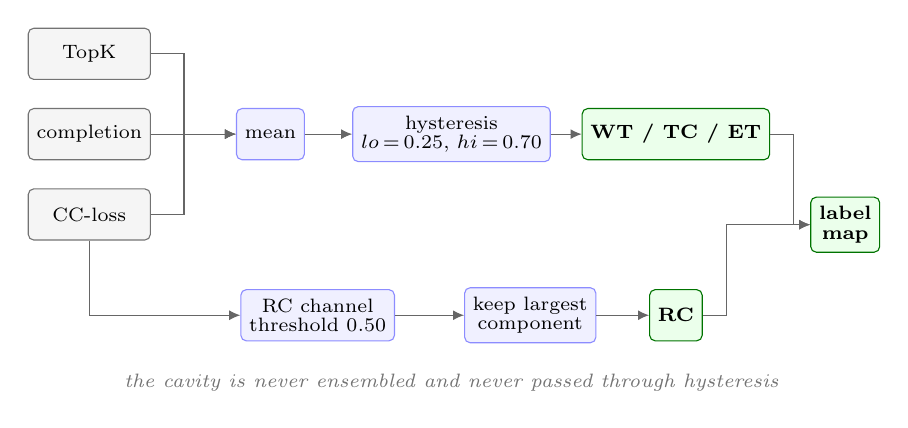
\begin{tikzpicture}[
  font=\scriptsize,
  box/.style   = {draw=black!55, rounded corners=2pt, align=center,
                  minimum height=6.5mm, inner xsep=3pt, fill=white},
  model/.style = {box, fill=black!4, minimum width=15.5mm},
  op/.style    = {box, fill=blue!6, draw=blue!45},
  fin/.style   = {box, fill=green!8, draw=green!45!black, font=\scriptsize\bfseries},
  ar/.style    = {-{Latex[length=4pt,width=3.6pt]}, draw=black!60},
]

% ---- ensemble members ------------------------------------------------------
\node[model] (m1) at (0,1.02)  {TopK};
\node[model] (m2) at (0,0)     {completion};
\node[model] (m3) at (0,-1.02) {CC-loss};

% ---- tumour path -----------------------------------------------------------
\node[op]  (mean) at (2.30,0)   {mean};
\node[op]  (hyst) at (4.60,0)   {hysteresis\\[-1pt] $lo\,{=}\,0.25$, $hi\,{=}\,0.70$};
\node[fin] (tum)  at (7.45,0)   {WT / TC / ET};

\draw[ar] (m1.east) -- ++(0.42,0) |- (mean.west);
\draw[ar] (m2.east) -- (mean.west);
\draw[ar] (m3.east) -- ++(0.42,0) |- (mean.west);
\draw[ar] (mean) -- (hyst);
\draw[ar] (hyst) -- (tum);

% ---- cavity path -----------------------------------------------------------
\node[op]  (rcth)  at (2.90,-2.30) {RC channel\\[-1pt] threshold $0.50$};
\node[op]  (rckp)  at (5.60,-2.30) {keep largest\\[-1pt] component};
\node[fin] (rc)    at (7.45,-2.30) {RC};

\draw[ar] (m3.south) |- (rcth.west);
\draw[ar] (rcth) -- (rckp);
\draw[ar] (rckp) -- (rc);

% ---- merge -----------------------------------------------------------------
\node[fin] (seg) at (9.60,-1.15) {label\\[-1pt] map};
\draw[ar] (tum.east) -- ++(0.30,0) |- (seg.west);
\draw[ar] (rc.east)  -- ++(0.30,0) |- (seg.west);

\node[align=center,black!55] at (4.60,-3.15)
  {\itshape the cavity is never ensembled and never passed through hysteresis};

\end{tikzpicture}
\caption{The submitted pipeline. Tumour regions are the unweighted mean of three members'
probability maps decoded by hysteresis; the cavity comes from the CC-loss member alone. The two
compose into one label map by painting WT, TC, ET, then RC, so nested regions overwrite parents.}
\label{fig:pipeline}
\end{figure}

Both thresholds were selected on the local harness of Section~\ref{sec:harness} and confirmed on
the official validation set. All code, the exact decode, the container definition and the
diagnostic scripts behind every number in this paper are released. Inference is deterministic
given the checkpoints; the submitted container bakes in all three and requires approximately
22\,s per case on a consumer GPU.

%%%%%%%%%%%%%%%%%%%%%%%%%%%%%%%%%%%%%%%%%%%%%%%%%%%%%%%%%%%%%%%%%%%%%%%%%%%%%%%
\section{Results}
\label{sec:results}

\subsection{Validation performance}

Table~\ref{tab:final} reports our best submission on the 179-case official validation set.

\begin{table}[t]
\centering
\caption{Best validation submission: three-way fusion, hysteresis $lo=0.25$, $hi=0.70$.
Official lesion-wise metrics, 179 cases.}
\label{tab:final}
\begin{tabular}{@{}lcccc@{}}
\toprule
 & WT & TC & ET & RC \\
\midrule
Lesion-wise Dice     & 0.725 & 0.766 & 0.746 & 0.630 \\
Lesion-wise NSD      & TODO  & TODO  & TODO  & TODO  \\
Small-instance $F_1$ & 0.376 & 0.478 & 0.476 & \textbf{0.167} \\
\bottomrule
\end{tabular}
\end{table}

Performance is markedly uneven across metric families. Overlap and surface metrics are strong,
while the three tumour $F_1$ cells sit far below at 0.376 to 0.478: roughly half of all lesion
instances are still missed or spuriously introduced, even where the lesions we do find are well
delineated. Detection, not delineation, is the residual problem, and the rest of this paper is
about why it resists the obvious fixes.

\paragraph{On uncertainty and significance.} We report point estimates without confidence
intervals, which is a genuine limitation rather than an oversight: the challenge server returns
only aggregate validation scores, and per-case metrics and reference labels are withheld from
participants, so dispersion and paired significance tests cannot be computed there at all. Where
we control the evaluation we report per-case counts instead. Readers should treat differences
below roughly 0.005 Dice as within our resolution to distinguish submissions.

\subsection{Ablation}
\label{sec:ablation}

\begin{table}[t]
\centering
\caption{Development path. All rows are our own submissions scored on the official 179-case
validation set, and are therefore directly comparable.}
\label{tab:ablation}
\begin{tabular}{@{}llcc@{}}
\toprule
 & change & Dice wt/tc/et & $F_1$ wt/tc/et \\
\midrule
1 & baseline nnU-Net ResEnc-L      & .560/.622/.593 & .379/.469/.463 \\
2 & \textbf{+ ensembling}          & .666/.708/.684 & .368/.439/.436 \\
3 & + second member, step 0.25     & .678/.718/.696 & .370/.477/.484 \\
4 & + RC from the CC-loss member   & .679/.719/.696 & .370/.477/.484 \\
5 & \textbf{+ hysteresis}          & .711/.753/.729 & .365/.468/.475 \\
6 & + third member                 & .720/.761/.737 & .376/.479/.477 \\
7 & + extent $lo$ 0.30 $\to$ 0.25  & \textbf{.725/.766/.746} & .376/.478/.476 \\
\bottomrule
\end{tabular}
\end{table}

Two steps dominate Table~\ref{tab:ablation}. Ensembling contributes $+0.106/+0.086/+0.091$ Dice
and hysteresis a further $+0.032/+0.034/+0.033$; together they account for $+0.138/+0.120/+0.124$
of the $+0.165/+0.144/+0.153$ total, or over four fifths of it. Both are inference-time operations
on frozen probability maps. The tumour $F_1$ column tells a complementary story: neither step
improves it, and the detection gains arrive only with the high-recall third member, which is
precisely the tension Section~\ref{sec:frontier} quantifies. Over the same period the components that cost most
to develop contributed nothing that survived. A tumour-specialist and a cavity-specialist model
were each \emph{worse} than the general network at their own speciality. A distance/boundary
loss, Laplacian-of-Gaussian hint channels, MedNeXt-v2, KiU-Net, U-Mamba and larger kernels were
all abandoned after failing to beat the baseline. We also determined that ``ResEnc-XL'' and
``ResEnc-L'' instantiate an identical network for this dataset, the planners differing only in
memory target, so architecture scaling is not a decorrelation lever here.

\subsection{The Dice--$F_1$ trade-off}
\label{sec:frontier}

Interpolating the fusion weight of the high-recall CC-loss member traces a strict trade-off
(Table~\ref{tab:frontier}). $F_1$ can be bought, but only by paying Dice, and the exchange rate is
unfavourable: moving from weight $1/3$ to $1/2$ buys $+0.053/+0.051/+0.066$ $F_1$ at a cost of
$-0.050/-0.046/-0.046$ Dice across three regions and eight of the twelve official metrics. We
retained $1/3$, the operating point at which the aggregate over all twelve official metrics was
best.

\begin{table}[t]
\centering
\caption{Fusion weight of the CC-loss member, on the official validation set. The trade is
monotone: every gain in detection is paid for in delineation.}
\label{tab:frontier}
\begin{tabular}{@{}lcc@{}}
\toprule
CC-loss weight & Dice wt/tc/et & $F_1$ wt/tc/et \\
\midrule
$1/3$ (submitted) & \textbf{.720/.761/.737} & .376/.479/.477 \\
$0.42$            & .695/.738/.714 & .403/.504/.510 \\
$1/2$             & .670/.715/.691 & \textbf{.429/.530/.543} \\
\bottomrule
\end{tabular}
\end{table}

The same trade separates our two thresholds, which are \emph{not} interchangeable knobs. Lowering
the seed threshold $hi$ from 0.70 to 0.65 gained $F_1$ $+0.042/+0.039/+0.043$ and lost Dice
$-0.017$: a large move along the trade-off, and one we rejected. Lowering the extent threshold
$lo$ from 0.30 to 0.25 gained Dice $+0.005/+0.005/+0.009$ for $-0.001$ $F_1$---not a move along
the trade-off at all, but a free gain, and the configuration we submitted. Pushing further to
$lo=0.20$ returned to trading, adding $+0.003/+0.002/+0.002$ Dice for $-0.003$ $F_1$ on whole
tumour, which brackets the useful range of the extent threshold at $lo=0.25$.

%%%%%%%%%%%%%%%%%%%%%%%%%%%%%%%%%%%%%%%%%%%%%%%%%%%%%%%%%%%%%%%%%%%%%%%%%%%%%%%
\section{Discussion}
\label{sec:discussion}

\subsection{The false positives are confident, which closes the obvious remedies}
\label{sec:fp}

Measured on 80 reference cases with the official metric, the median peak probability inside a
false positive is \textbf{0.96}, while inside a lesion we miss it is \textbf{0.55}. We detect 45\%
of small lesions; 43\% of the misses are ones the model is wholly blind to, never exceeding a
probability of 0.10 anywhere inside them; and 86\% of false positives fall far from any reference
lesion.


\textbf{The model is more confident about its mistakes than about the lesions it finds.} Its
false positives are additionally spatially coherent---they survive Gaussian smoothing as solid
blobs rather than dissolving as noise would---isolated, and \emph{corroborated}: they survive
averaging across three independently trained networks because all three fire on them.

This one fact refutes seven suppression mechanisms (Table~\ref{tab:refuted}), each of which
separates on confidence or on a quantity monotone in it. We report them because the failure is
systematic rather than incidental, and because several are standard practice a reader would
otherwise reasonably try. The pattern across the middle column is the finding: the per-component
loss penalty collapsed into global under-confidence, and the learned veto never learned what a
false positive looks like, for the reason this section documents---they look like lesions.

\begin{table}[t]
\centering
\caption{The seven refuted false-positive suppression mechanisms. The middle column is the
point: every one of them ranks candidate components by confidence, or by a quantity monotone in
it, and our false positives sit at the confident end.}
\label{tab:refuted}
\small
\setlength{\tabcolsep}{4pt}
\renewcommand{\arraystretch}{1.15}
\begin{tabular}{@{}>{\raggedright\arraybackslash}p{0.235\textwidth}
                  >{\raggedright\arraybackslash}p{0.165\textwidth}
                  >{\raggedright\arraybackslash}p{0.555\textwidth}@{}}
\toprule
mechanism & separates on & outcome \\
\midrule
small-component filters      & size            & annihilated $F_1$; small \emph{is} real \\
\addlinespace[1.5pt]
rejection by mean confidence & mean prob.      & recovered Dice, destroyed the recall it was
                                                 meant to preserve \\
\addlinespace[1.5pt]
per-component FP penalty in the loss & component prob. & FP $-53\%$ but TP $-24\%$; collapsed
                                                 into global under-confidence \\
\addlinespace[1.5pt]
the same model as a learned veto & learned prob. & at $t=0.5$ it rejected \emph{everything}
                                                 (TP $1.82\to0.51$) \\
\addlinespace[1.5pt]
blending the veto with the base & mixture of both & FPs and TPs removed in lockstep at every
                                                 mixing ratio \\
\addlinespace[1.5pt]
size-adaptive seed threshold & size $\times$ prob. & reproduces the plain global threshold
                                                 exactly \\
\addlinespace[1.5pt]
scale-space (smoothed) seed  & smoothed prob.  & at every matched FP rate the plain threshold
                                                 detects more \\
\bottomrule
\end{tabular}
\end{table}

\subsection{Mimics, not annotation gaps---and still not separable}

Two explanations remained. Either these are anatomical \emph{mimics}---enhancing vessels, choroid
plexus, dural structures---that a radiologist excludes using context the network lacks, or they
are \emph{real metastases the annotators missed}, in which case part of the ceiling is not ours
to move.

Visual review of the 48 most confident false positives favours the mimic hypothesis. They are
overwhelmingly small bright enhancing foci in three anatomically suspicious locations: at the
cortical margin or dura, on or beside bright linear tubular structures consistent with vessels,
and at the midline in falx and superior sagittal sinus territory. Few resemble what an annotation
gap would look like, namely an isolated round parenchymal lesion in otherwise uniform white
matter.

Anatomical position is a genuinely different separation axis from confidence, so we measured it
rather than trusting the impression. Distance from the brain surface to the false-positive
centroid has a median of 8.8\,mm against 11.2\,mm for reference lesion centroids, with almost
fully overlapping interquartile ranges and an area under the ROC curve of \textbf{0.575}. False
positives are only marginally more peripheral, and grey--white junction metastases---a common
true presentation---sit at the same depth, so any filter aggressive enough to remove the mimics
removes real lesions with them. The axis is measurable, real, and useless.

\subsection{Two attempts to fix detection during training}

Since decoding could not separate these errors, we attacked the 43\% of misses to which the
network is wholly blind from the training side.

\paragraph{Oversampling small lesions failed.} nnU-Net's sampler draws a random key from
\texttt{class\_locations} and then a random voxel within it, so a thirty-voxel metastasis sharing
a key with every large-lesion and oedema voxel is patch-centred approximately 0.3\% of the time.
We added a dedicated key containing only small-component voxels, with every lesion weighted
equally regardless of size. Verified over 4000 draws, the probability of centring a patch on a
small lesion rose from 1.28\% to 25.75\%, a twenty-fold increase. \emph{The blindness did not
move.} The network is not blind to small metastases because it rarely sees them, and starvation
can be excluded as the mechanism.

\paragraph{Enlarging the target worked, but could not be banked.} We instead dilated isolated
small targets, so a thirty-voxel lesion presents roughly four times the volume and a larger
object for the receptive field, with a matched selective erosion at inference. Submitted alone
this lifted tumour $F_1$ by $+0.012/+0.014/+0.013$, evidence that a meaningful share of the extra
detections are real. Grafting only the additional, non-overlapping detections onto our best
submission raised $F_1$ by as much as $+0.034/+0.027/+0.031$ but lowered lesion-wise Dice by
$-0.010/-0.012/-0.012$. The net effect across the official metrics was negative. The reason is specific to lesion-wise scoring and
worth stating plainly: \emph{every newly detected small lesion enters the per-lesion Dice average
at a below-average value}, because small lesions are segmented less accurately than large ones.
Under volumetric Dice the graft would be nearly free; under lesion-wise Dice it is not. A more
aggressive variant added 156 further components averaging six voxels each and bought only
$+0.003/+0.004/+0.005$ $F_1$, indicating that the smallest specks are overwhelmingly mimics.

\subsection{A limit on tuning post-processing with a memorised model}
\label{sec:harness}

We built a local harness around the official evaluation code over 80 reference tumour cases and
100 cavity cases, gated on reproducing the relative ordering of our own previously scored
submissions. It replaced blind two-submissions-per-day guessing---during which $F_1$ moved
$+0.001$ in ten days---and selected our best submission from 28 candidate decodes at no
submission cost. It also has a failure mode we did not anticipate, and which applies to any team
tuning post-processing on models trained without a held-out fold.

Every model was trained on these cases. For decodes---the same probabilities post-processed
differently---this is tolerable, because memorisation is common-mode and largely cancels from a
\emph{ranking} of candidates. It is not tolerable for a rule that changes \emph{how many
components are kept}. On memorised cases the model rarely emits a spurious component, since it
knows the answer, so a ``keep more components'' rule appears free, with true positives rising and
false positives flat. On unseen data the model does emit such components and the same rule admits
them. \textbf{Memorisation suppresses precisely the false positives that the rule would let in,
so the harness is structurally blind to its cost.}

The effect is not small. A cavity keep-rule measured locally at $+0.028$ lesion-wise Dice
delivered $-0.016$ on the validation set---the wrong \emph{sign}, not merely the wrong magnitude.
More broadly the harness consistently overestimated the size of the gains it predicted, by
roughly a factor of three. Our operating rule became: thresholds and fusion weights may be tuned offline,
because they change values rather than counts; component filters, keep-rules and size cutoffs may
not, and must be validated on a real submission or a genuine held-out fold.

\subsection{Limitations}
\label{sec:limits}

All models are trained without a held-out fold, which is the root cause of the harness limitation
above and the reason our offline forecasts are optimistic by roughly a factor of three. A single
held-out-fold run would fix this permanently and would additionally supply a decorrelated
ensemble member; we exhausted our compute budget before it was possible. Our members share a
lineage, which is why they corroborate one another's false positives and why adding a fourth
member of the same lineage did not help. As noted in Section~\ref{sec:results}, we cannot report
dispersion or significance on the validation set because per-case scores are not returned to
participants. The visual review of false positives was performed by a non-radiologist on single
axial slices and should be read as the hypothesis that the surface-distance measurement was
designed to test, not as a clinical assessment. Finally, all findings are specific to
lesion-wise scoring on this cohort; the frontier of Section~\ref{sec:frontier} would look
entirely different under a volumetric metric.

%%%%%%%%%%%%%%%%%%%%%%%%%%%%%%%%%%%%%%%%%%%%%%%%%%%%%%%%%%%%%%%%%%%%%%%%%%%%%%%
\section{Conclusion}
\label{sec:conclusion}

Our BraTS 2026 Task 1 submission reaches lesion-wise Dice of 0.725/0.766/0.746 with no novel
architecture and no novel loss, using ensembling as false-positive dilution and hysteresis
decoding. Our residual deficit is entirely in tumour detection $F_1$, and we have shown it is not
addressable by confidence-based suppression, that the false positives are anatomical mimics which
are nonetheless not separable by anatomical position, and that lesion-wise Dice actively penalises
recovering additional small lesions. We hope these negative results prove as useful as the method
itself. All code is released at \url{https://github.com/aymuos15/brats2026-mets}.

\subsubsection{Acknowledgements.} Data used in this publication were obtained as part of the
Challenge project through Synapse ID (syn74274097).

\begin{thebibliography}{8}

\bibitem{baid2021}
Baid, U., et al.: The RSNA-ASNR-MICCAI BraTS 2021 benchmark on brain tumor segmentation and
radiogenomic classification. arXiv:2107.02314 (2021)

\bibitem{bratsmet2023}
Moawad, A.W., et al.: The Brain Tumor Segmentation (BraTS-METS) challenge 2023: brain metastasis
segmentation on pre-treatment MRI. arXiv:2306.00838 (2023)

\bibitem{medperf2023}
Karargyris, A., Umeton, R., Sheller, M.J., et al.: Federated benchmarking of medical artificial
intelligence with MedPerf. Nature Machine Intelligence \textbf{5}, 799--810 (2023)

\bibitem{isensee2021nnunet}
Isensee, F., Jaeger, P.F., Kohl, S.A.A., Petersen, J., Maier-Hein, K.H.: nnU-Net: a
self-configuring method for deep learning-based biomedical image segmentation. Nature Methods
\textbf{18}(2), 203--211 (2021)

\bibitem{isensee2024resenc}
Isensee, F., et al.: nnU-Net revisited: a call for rigorous validation in 3D medical image
segmentation. In: MICCAI 2024. Springer (2024)

\bibitem{kofler2022blob}
Kofler, F., et al.: blob loss: instance imbalance aware loss functions for semantic segmentation.
In: IPMI 2023. Springer (2023)

\bibitem{canny1986}
Canny, J.: A computational approach to edge detection. IEEE Transactions on Pattern Analysis and
Machine Intelligence \textbf{8}(6), 679--698 (1986)

\bibitem{kundu2026instance}
Kundu, S.S., Kofler, F., Ivory, M., M\"oller, H., Shapey, J., Vercauteren, T.: Instance awareness
of multi-class semantic segmentation loss functions. arXiv:2604.24276 (2026)

\bibitem{grosskopf2026matching}
Gro\ss{}kopf, E., Kundu, S.S., M\"oller, H., M\"unster, N., Astaraki, M., Buzduga, P.T., Ritter, K.,
Wiestler, B., Kirschke, J., Shapey, J., Vercauteren, T., Kofler, F.: Redefining instance matching:
a unified framework for part-aware matching in panoptic segmentation evaluation.
arXiv:2605.31094 (2026)

% TODO: the organisers will release the BraTS 2026 challenge manuscript and require it to be
% cited. Re-check the Challenge Rules wiki page (syn74274097 / 639585) before camera-ready.

\end{thebibliography}

\end{document}
